\chapter{Eulerian Domain: Finite Element Method}

	\lsymb[f]{$\mathcal{T}_h$}{Finite Element mesh}{-}{th}		
	\lsymb[f]{$T$}{Cell of Finite Element mesh}{-}{t}			
	
	\lsymb[f]{$v$}{Test function}{-}{v}				
	\lsymb[f]{$V$}{Trial vector function space}{-}{vte}				
	\lsymb[f]{$\hat{V}$}{Test vector function space}{-}{vtr}					
	\gsymb[f]{$\Omega$}{Fluid domain}{-}{x}	
	\gsymb[f]{$\Omega_E$}{Eulerian fluid domain}{-}{xe}	
	\gsymb[f]{$\Omega_L$}{Lagrangian fluid domain}{-}{xl}	
	\gsymb[f]{$\partial \Omega$}{Boundary of the domain $\Omega$}{-}{xdd}	

%------------------------------------------------------------------------------------------------------
%------------------------------------------------------------------------------------------------------
%------------------------------------------------------------------------------------------------------
%\section{Purpose of eulerian domain}
Standard \printAcron{Computation Fluid Dynamics}{CFD} method discretizes the fluid into smaller regions, known as grids, and solves the set of Navier-Stokes equations in this region. This type of formulation is referred to as Eulerian method as we are evaluating the change of flow property in a given volume.

For the hybrid method, we use the Navier-Stokes grid formulation in the near-body region. The advantage of using the Eulerian method at this region is that it is much more efficient in resolving the boundary layer than the typical Vortex Particle Method. We can directly enforce the wall boundary condition at the wall boundary of the Eulerian domain, solving the problem of vorticity generation from a body. In the hybrid coupling strategy, we will interpolate this newly resolved near-wall solution on to the Lagrangian domain, where the vortex blobs will efficiently evolve the particles from the Lagrangian frame point.

The various approaches to solve the fluid dynamics problem from a Eulerian reference frame. \indexAcron{Finite Volume Method }{FVM}, \indexAcron{Finite Difference Method}{FDM}, and \indexAcron{Finite Element Method}{FEM} are the common choice for solving the Navier-Stokes problem and differ by the way they approach to solve the problem. FVM divides the domain into volumes where it enforces the conservation of mass and momentum in each sub-domains. FDM divides the domain into nodes and use local Taylor expansions to approximate the partial differential equations. FEM divides the domain into elements and solves the problem using variational calculus. So, in the end, the choice of Eulerian method does not have a direct impact on the coupling with the Lagrangian method. 

We have decided to use the FEM packages provided by the \texttt{FEniCS} project as they have be already implemented efficient, multi-threaded algorithms for solving differential equation and provide extensive features for future developments such as adaptive mesh refinement, fluid-structure interaction, and efficient computation of turbulence.

\section{Introduction to Finite Element Method}

\printAcron{Finite Element Method}{FEM} is numerical method to solve for the solution of a given differential equation. It is solved by describing it as a variation problem, and by minimizing the error we can reach a approximate solution for the problem \cite{Brenner2008}. So, the FEM approximates the unknown variables and converts the partial differential equations to algebraic equations. It was traditionally used for solid mechanics, for the analysis of aircraft structures \cite{Rao2005}, but have since then used to solve the Navier-Stokes fluid dynamics problems \cite{Guermond2006} \cite{Johnston2004} \cite{Guermond2003}.

\subsection*{Finite element discretization}

	\begin{figure}[!t]
	\centering
	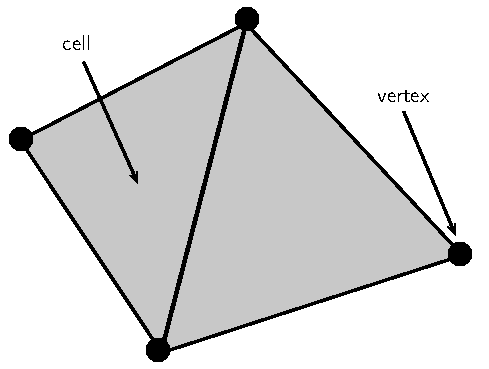
\includegraphics[width=0.4\linewidth]{./figures/eulerian/finiteElementDefinitions.pdf}
	\caption{A two-dimensional Finite Element geometry. The cell represents the area of the element, and vertices are the edge of the cell.}
	\label{fig:finiteElementDefinitions}
	\end{figure}

\begin{figure}[!b]
        \centering
        \begin{subfigure}[b]{0.5\textwidth}
                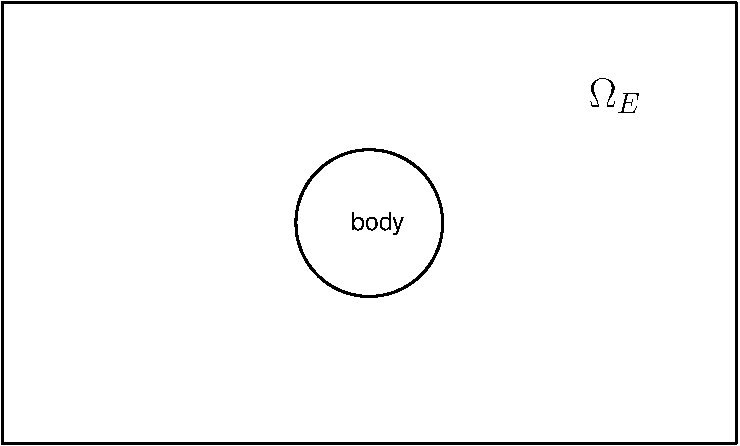
\includegraphics[width=\textwidth]{figures/eulerian/cylinderPreDelauney-crop.pdf}
                \caption{Fluid domain $\Omega_E$ around the cylinder}
                \label{fig:cylinderPreDelauney}
        \end{subfigure}%
        ~ %add desired spacing between images, e. g. ~, \quad, \qquad etc.
          %(or a blank line to force the subfigure onto a new line)
        \begin{subfigure}[b]{0.5\textwidth}
                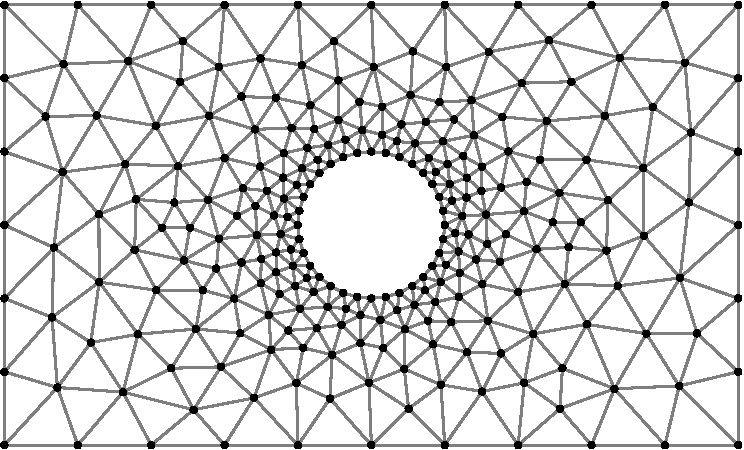
\includegraphics[width=\textwidth]{figures/eulerian/cylinderDelauney-crop.pdf}
                \caption{Delaunay triangulation of the fluid}
                \label{fig:cylinderDelauney}
        \end{subfigure}
        \caption{Delaunay triangulation of the fluid around a cylinder resulting in unstructured mesh with controllable cell sizes.}
        \label{fig:cylinderFiniteElementDiscretization}
\end{figure}	
	
Finite Element solves by dividing the domain of interest into small, simple regions known as ``finite elements". These ``elements" are connected at the joints and are called nodes or nodal points. We use these sets of node and elements to represent the actual variation in the field (such as displacement, velocity, pressure or temperature) using simple functions, known as basis functions. Therefore, we have transformed a domain of infinite \indexAcron{Degrees of Freedom}{DOF} to a finite number of DOFs. We combine this set of equations of element equations into a global system of equations to solve for the final problem.

The discretization of a 2D domain can be observed in figure \ref{fig:finiteElementDefinitions}. The figures shows two connect finite elements. The cells represent the area of the element, and vertices of the cell are the node of the finite element. Therefore, we have divide the domain $\Omega$ into finite sets of cells $\mathcal{T}_h = \{T\}$ and together these cells make the mesh of the Eulerian domain. As seen in figure \ref{fig:finiteElementDefinitions}, the cells are made of simple geometrical shapes (in 2D): triangles, quadrilaterals, tetrahedrals and so on. The common approach to divide the domain is use to use triangles as the the basic geometry. Figure \ref{fig:cylinderFiniteElementDiscretization} shows the discretization of the fluid domain around a cylinder using Delaunay triangulation. This type of discretization results in unstructured mesh and is advantageous when we have to deal will complicated geometries. 

\subsection*{Finite element function and function space}

When the domain $\Omega$ is divided into cells $T$, we can define the function and the function space of the Finite element problem. For each cell, a local function space $\mathcal{V}$ can be defined to collectively construct the global function space $V$.

To solve a basic problem such as a Poisson equation numerically, we need to convert it into a variational problem. A 1D Poisson problem is given as,

	\begin{subequations}
	\begin{align*}
	- \nabla^2 u(x) &= f(x), \qquad x\ \mathrm{in}\ \Omega,\\
	u(x) &= u_0(x), \qquad x\ \mathrm{on}\ \partial\Omega.
	\end{align*}
	\label{eq:poissonEq}
	\end{subequations}
	
We can transform equation \ref{eq:poissonEq} into the variational form by multiplying with a test function $v$, and integrating it over the domain $\Omega$,


	\begin{equation}
	- \int_{\Omega} \left(\nabla^2 u\right)v\ \mathrm{d}x= \int_{\Omega} fv\ \mathrm{d}x.
	\label{eq:poissonEqVariationFormA}
	\end{equation}

The function $u$ in variational form, equation \ref{eq:poissonEqVariationFormA}, is known as the trial function and it is the solution that we are trying to approximate. The test function $v$ lies in the test function space $\hat{V}$ and our trial function $u$ lies on the function space $V$. When performing integration by parts, the test function $v$ is required to be zero at regions where $u$ is known. So, the additional terms cancel and we get,

	\begin{equation}
	- \int_{\Omega} \nabla u \nabla v\ \mathrm{d}x= \int_{\Omega} fv\ \mathrm{d}x.
	\label{eq:poissonEqVariationFormB}
	\end{equation}

This form is referred to as the ``weak-form" of the original Poisson equation and in order to solve this continuous problem numerically, we must discretize it first into discrete variational problem.


%------------------------------------------------------------------------------------------------------
%------------------------------------------------------------------------------------------------------
%------------------------------------------------------------------------------------------------------
\section{Solving the Finite Element problem}

\subsection{Introduction to FEniCS Project}

\subsection{Mesh generation using GMSH}


%------------------------------------------------------------------------------------------------------
%------------------------------------------------------------------------------------------------------
%------------------------------------------------------------------------------------------------------
\section{Solving Incompressible Navier-Stokes Equations}

\subsection{Velocity-pressure formulation}

\subsection{Incremental pressure correction scheme}

\subsection{Determining the vorticity field}

\subsection{Determining the body forces}

\subsubsection*{Frictional Forces}

\subsubsection*{Pressure Forces}


\section{Validation of eulerian method}

%\subsection{Lamb-oseen vortex}

\subsection{Clercx-Bruneau dipole collison at $Re=625$}

\subsection{Impulsively started cylinder at $Re=550$}

\section{Summary}

